% (c) Egor Osipov

\documentclass[a4paper,12pt]{article} % тип документа (report, book)
\usepackage[14pt]{extsizes}
\usepackage[left=2cm,right=2cm, top=2cm,bottom=2cm,bindingoffset=0cm]{geometry} % Настройки документа
\usepackage{pgfplots}
\usepackage{pgfplotstable}
\usepackage{tikz} 

%  Русский язык
\usepackage[T2A]{fontenc}			% кодировка
\usepackage[utf8]{inputenc}			% кодировка исходного текста
\usepackage[english,russian]{babel}	% локализация и переносы


% Математика
\usepackage{amsmath,amsfonts,amssymb,amsthm,mathtools} 

% Просто смайлики
\usepackage{wasysym}

%Вставка картинок
\usepackage{graphicx}
\graphicspath{./}
\DeclareGraphicsExtensions{.pdf,.png,.jpg}
\usepackage{float}

% Настройка абзацев
\usepackage{indentfirst}
%\setlength{\parindent}{5ex}
%\setlength{\parskip}{1em}

\begin{document} % начало документа

%Заговолок
\begin{titlepage}
\begin{center}
	\large{Московский физико-технический институт}\\
	\vspace{100px}
	\LARGE{Лабораторная работа № 3.5.1.}\\
	\LARGE{Изучение плазмы газового разряда в неоне.}\\
	\vspace{30px}
	
\includegraphics[scale = 0.3]{fakt_logo.png}\\
\end{center}

\vfill
\begin{flushright}
	\text{Осипов Егор. Б03-005}\\
	\text{22.09.2021}\\
	\text{г. Долгопрудный}
\end{flushright}
\end{titlepage}

\newpage

\tableofcontents

\newpage

\textbf{Цель работы:} изучение вольт-амперной характеристики газового тлеющего разряда; изучение свойств плазмы методом зондовых характеристик.

\textbf{В работе используется:} стеклянная газоразрядная трубка, наполненная изотопом неона, высоковольтный источник питания, источник питания постоянного тока, делитель напряжения, резистор, потенциометр, амперметры, вольтметры, переключатель.

\section{Подготовка к работе.}
\subsection{Экспериментальная установка.}

Схема установки приведена на рисунке \eqref{ustanovka}. Стеклянная газоразрядная трубка имеет холодный (ненакаливаемый) полый катод, три анода и \textit{геттерный узел} - стеклянный баллон, на внутреннюю поверхность которого напылена газопоглащающая пленка (\textit{геттер}).
Трубка наполнена изотопом неона $^{22}\text{Ne}$ при давлении 2 мм.рт.ст. Катод и один из аннодов (\textbf{I} или \textbf{II}) с помощью переключателя $\text{П}_1$ подключаются через балластный резистор $R_\text{б} \simeq 450 \text{кОм}$ к регулярному высоковольтному источнику питания (ВИП) с выходным напряжением до 3 кВ.

\begin{figure}[H]\label{ustanovka}
	\center{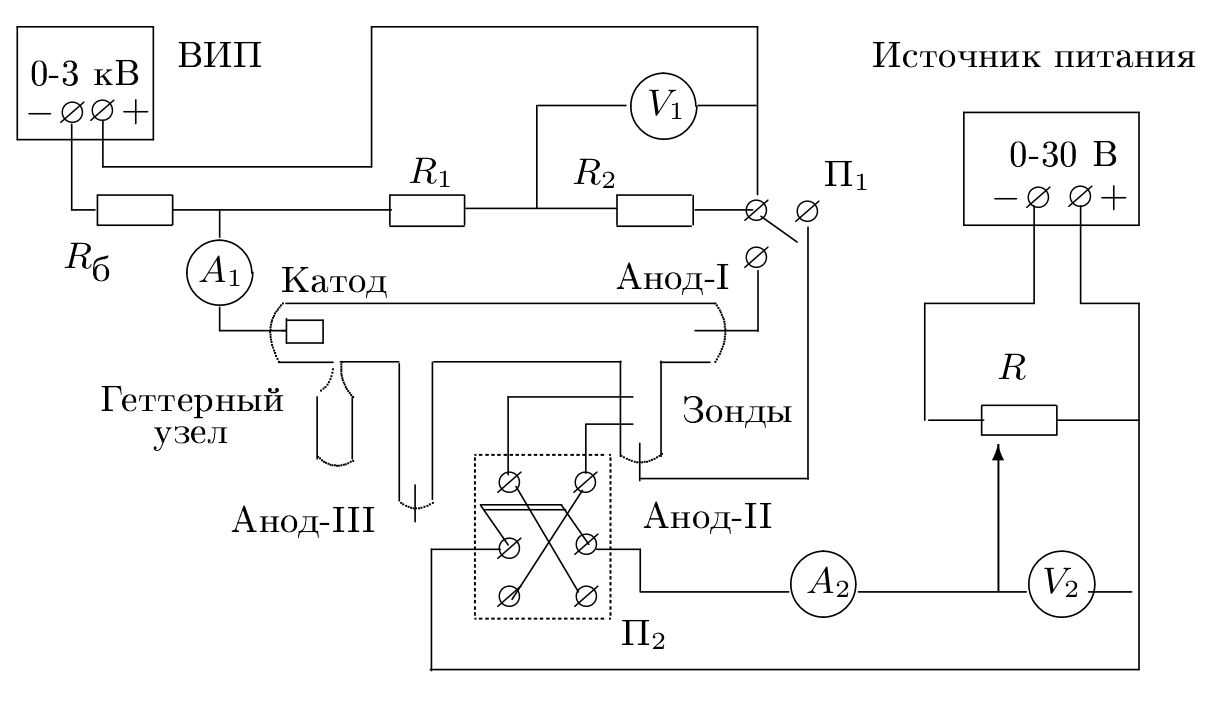
\includegraphics[scale=0.4]{ustanovka}}
	\caption{Схема установки для исследования газового разряда.}
\label{fig:image}
\end{figure}

При подключении к ВИП аннода \textbf{I} между ним и катодом возникает газовый разряд. Ток разряда измеряется миллиамперметром $\text{\textbf{A}}_1$, а падение напряжения на разрядной трубке -- цифровым вольтметром $\text{\textbf{V}}_1$, подключенный к трубке через высокоомный (25 МОм) делитель напряжений с коэффициентом $(R_1 + R_2) / R_2 = 10$.

При подключении к ВИП аннода \textbf{II} разряд возникает между катодом и аннодом \textbf{II}, где назодится двойной зонд, используемый для диагностики плазмы положиетльного столба. Зонды изготовлены из молибденовой проволоки диаметром $d = 0.2\text{мм}$ и имеют длину $l = 5.2\text{мм}$. Они подключены к источнику питания через потенциометр \textbf{R}. Переключатель $\text{\textbf{П}}_2$ позволяет изменять полярность напряжений на зондах. Величина напряжений на них изменяется с помощью дискретного переключателя <<\textbf{\textit{V}}>> выходного  напряжения источника питания и потенциометра \textbf{R} и измеряется вольтметром $\text{\textbf{V}}_2$. Для измерения зондового тока используется микроамперметр $\text{\textbf{A}}_2$.

Аннод-\textbf{III} в работе не используется.

\section{Задача.}

\subsection{Предполагаемый ход выполнения.}

В работе предлагается снять вольт-маперную характеристику тлеющего разряда и зондовые характеристики при разных токах разряда и по результатам измерений расчитать концентрацию и температуру электронов в плазме, степень ионизации, плазменную частоту и дебаевский радиус экранирования.

1. Снимем вольт-амперную характеристику разряда. Для этого: установим переключатель $\text{\textbf{П}}_1$ в положение <<Анод-\textbf{I}>>; ручку регулировки входного напряжени ВИП - на минимум; включим ВИП в сеть. Плавно увеличивая выходное напряжение ВИП, определим напряжение зажигания заряда, снимем зависимость напряжения $\text{\textit{U}}_1$ на разрядной трубке от протекающего в ней тока $\text{\textit{I}}_\text{р}$. Ток разряда изменяем в диапазон от 0.5 до 5 мА.

2. Снимем зондовые характеристики. Уменьшим напряжение ВИП до 0, переведем переключатель $\text{\textbf{П}}_1$ в положение <<Анод-\textbf{II}>> и будем плавно увеличивать напряжение ВИП до возникновения разряда. Установим разрядный ток $\text{\textit{I}}_\text{р} = 1 \text{мА}$. Включим источник питания постоянного тока Б5-47 и снимем вольт-амперную характеристику двойного разряда $\text{I} = f(\text{U})$. Повторим измерения при другой полярности (переключатель $\text{\textbf{П}}_2$).

Повторим измерения зондовых характеристик при токах разряда равных 2, 3, 4 и 5 мА.

\subsection{Заметки по теории.}

Дебаевский радиус характеризует жкранирование ионов электронами, в следствии чего потенциал исчисляется по формуле \eqref{5.11}.

\textbf{Плазмой называется ионизированный газ, дебаевский радиус которого $r_D$ существенно меньше характерного размера \textit{l} объема, занимаемого этим газом.}

$N_D$ - число частиц в дебаевской сфере. Для плазмы газового разряда это примерно $10^4$. Формула \eqref{5.12}.

Плазменная (\textbf{ленгмюровская}) частота получается из смещения электронов относительно ионов в воображаемом параллепипеде. \textbf{Это время отклика на флуктуацию заряда в плазме.} В таком случае дебаевская частота -- это апмлитуда ленгмюровских колебаний плазмы.

\subsection{Формулы, которые могут понадобиться.}

\begin{equation}\label{5.11}
\varphi = \frac {Ze} {r} e^{-r / r_D}
\end{equation}

\begin{equation}\label{5.12}
N_D \approx n \frac{4}{3} \pi r^3_D \approx 0.1 \frac{(kT_e)^{3/2}}
{n^{1/2} e^3}
\end{equation}

\begin{equation}\label{5.43}
kT_e = \frac{1}{2} \frac{e I_{i\text{н}}} {\frac{dI}{dU}\vert_{U = 0}}
\end{equation}

\begin{equation}\label{5.31}
I_{i\text{н}} = 0.4n_e eS \sqrt{\frac{2kT_e}{m_i}}
\end{equation}

\begin{equation}\label{5.16}
\omega_p = \sqrt{ \frac{n_e e^2}{\epsilon_0 m_e} }
\end{equation}


Дебаевский радиус $r_d$

\begin{equation}\label{5.18}
r_d = \sqrt{ \frac{\epsilon_0 K T_i}{n e^2} }
\end{equation}

\section{Результаты эксперимента и их обработка.}

Приведем таблицу зависимости вольт-амперной характеристики заряда

\begin{table}[H]
\caption{\label{tab:canonsummary} Вольт-амперная характеристика разряда.}
\begin{center}
\begin{tabular}{|c|c|c|c|c|c|c|c|c|c|}
\hline
U В & 30.93 & 30.59 & 30.35 & 30.25 & 30.42 & 30.31 & 31.46 & 34.19 & 36.71\\
\hline
I мА & 2.09 & 2.61 & 3.37 & 5.11 & 4.45 & 3.17 & 1.70 & 0.74 & 0.17\\
\hline
\end{tabular}
\end{center}
\label{table1:ref}
\end{table}

\begin{figure}[H]\label{rlx}
	\center{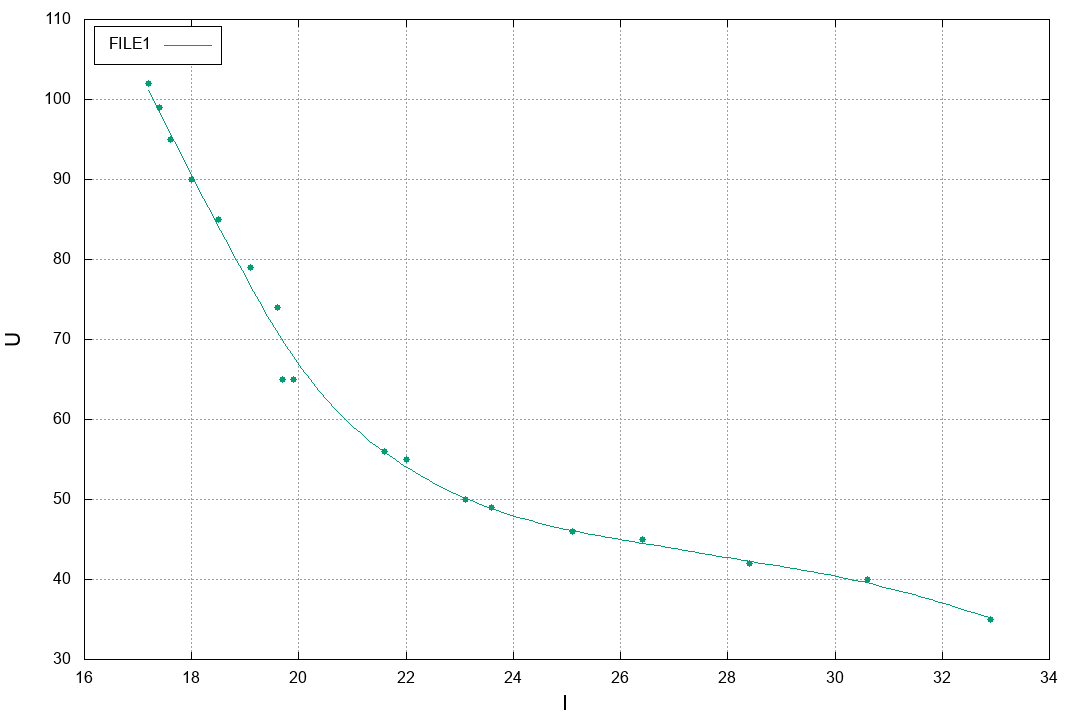
\includegraphics[scale=0.6]{1st_graph}}
 	\caption{Вольт-амперная характеристика разряда.}
\label{fig:image}
\end{figure}

%\begin{table}[H]
%\begin{center}
%\caption{\label{tab:res2} Зондовые характеристики ($I_p = 5\text{мА}$, $I_p = 3\text{мА}$, $I_p = 1.5\text{мА}$)}
%\begin{tabular}{|c|c|}
%\hline
%U(В) & I(мкА) \\ \hline
%25.0 & 120.0 \\ \hline
%22.0 & 117.3 \\ \hline
%19.1 & 114.2 \\ \hline
%16.0 & 109.9 \\ \hline
%13.1 & 103.2 \\ \hline
%10.1 & 93.3 \\ \hline
%8.2 & 82.0 \\ \hline
%5.98 & 67.6 \\ \hline
%4.1 & 52.1 \\ \hline
%2.0 & 33.7 \\ \hline
%-25.0 & -115.0 \\ \hline
%-22.2 & -112.5 \\ \hline
%-19.1 & -109.6 \\ \hline
%-16.0 & -105.4 \\ \hline
%-13.1 & -99.1 \\ \hline
%-10.1 & -88.8 \\ \hline
%-8.0 & -78.5 \\ \hline
%-6.1 & -65.8 \\ \hline
%-4.1 & -50.3 \\ \hline
%-2.1 & -32.3 \\ \hline
%-0.095 & -12.6 \\ \hline
%&\\ \hline
%\end{tabular}\;\;\;
%\begin{tabular}{|c|c|}
%\hline
%U(В) & I(мкА) \\ \hline
%25.0 & 60.1 \\ \hline
%22.2 & 58.6 \\ \hline
%19.3 & 56.9 \\ \hline
%16.1 & 55.0 \\ \hline
%13.2 & 52.6 \\ \hline
%10.1 & 47.9 \\ \hline
%8.2 & 43.2 \\ \hline
%5.9 & 35.0 \\ \hline
%4.2 & 26.8 \\ \hline
%2.1 & 15.6 \\ \hline
%0.006 & 2.3 \\ \hline
%-25.0 & -62.8 \\ \hline
%-2.0 & -14.2 \\ \hline
%-4.1 & -26.2 \\ \hline
%-6.1 & -35.9 \\ \hline
%-8.2 & -44.1 \\ \hline
%-9.9 & -49.0 \\ \hline
%-13.3 & -54.9 \\ \hline
%-16.4 & -57.6 \\ \hline
%-18.9 & -59.3 \\ \hline
%-22.3 & -61.3 \\ \hline
%-25.0 & -62.9 \\ \hline
%\end{tabular}\;\;\;
%\begin{tabular}{|c|c|}
%\hline
%U(В) & I(мкА) \\ \hline
%25.0 & 28.9 \\ \hline
%22.3 & 28.0 \\ \hline
%19.1 & 26.9 \\ \hline
%16.1 & 26.0 \\ \hline
%13.3 & 24.8 \\ \hline
%10.2 & 22.7 \\ \hline
%8.3 & 20.6 \\ \hline
%5.8 & 16.6 \\ \hline
%4.1 & 12.7 \\ \hline
%2.2 & 7.6 \\ \hline
%0.007 & 0.6 \\ \hline
%-0.007 & -0.01 \\ \hline
%-2.0 & -6.5 \\ \hline
%-4.1 & -12.3 \\ \hline
%-6.2 & -17.2 \\ \hline
%-8.1 & -20.1 \\ \hline
%-10.1 & -23.2 \\ \hline
%-13.2 & -25.2 \\ \hline
%-16.3 & -26.9 \\ \hline
%-19.1 & -27.9 \\ \hline
%-22.2 & -28.9 \\ \hline
%-25.0 & -29.9 \\ \hline
%\end{tabular}
%\end{center}
%\label{table2:ref}
%\end{table}

\begin{figure}[H]\label{rlx}
	\center{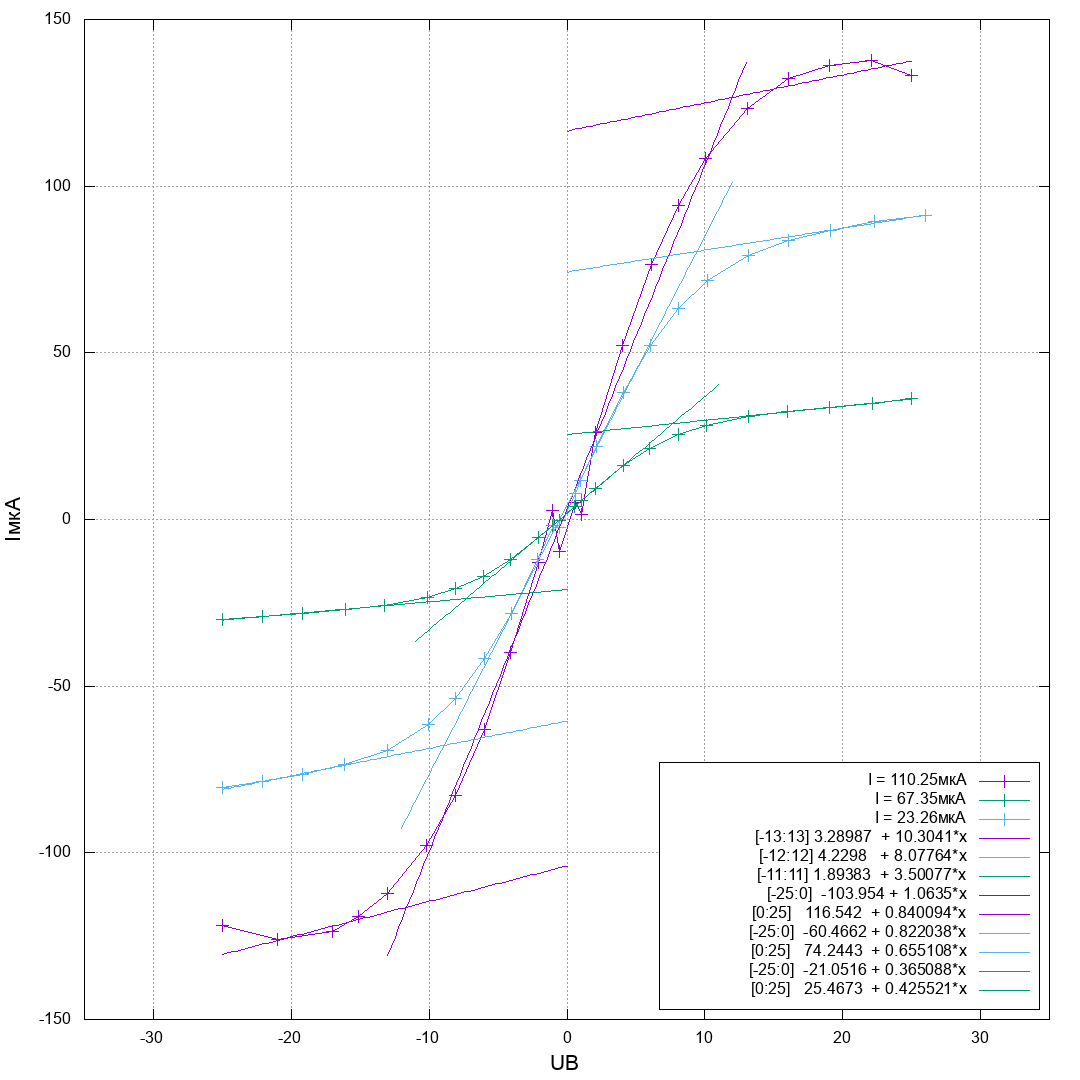
\includegraphics[scale=0.6]{2nd_plot}}
 	\caption{Зондовые характеристики.}
\label{fig:image2}
\end{figure}

Рассчитаем температуру электронов в электрон-вольтах, концентрацию электронов, плазменную частоту колебаний, дебаевский радиус и число электронов в дебаевской сфере по формулам:

\begin{equation}
    kT_e = \frac{1}{2}\cdot \frac{eI_{i\text{н}}}{\frac{\delta I}{\delta U}|_{U = 0}}\;\;\;\;\;n_e = \frac{I_{i\text{н}}}{0.4 eS}\sqrt{\frac{m_i}{2kT_e}}\;\;\;\;\;\omega_p = \sqrt{\frac{n_e e^2}{\varepsilon_0 m_e}}
    \label{eq3:ref}
\end{equation}

\begin{equation}
    r_D = \sqrt{\frac{\varepsilon_0kT_i}{ne^2}} \;\;\;\;\;  N_D = \frac{4}{3}n\pi r_D^3
    \label{eq4:ref}
\end{equation}

\begin{table}[H]
\caption{\label{tab:canonsummary} Рассчетные величины.}
\begin{center}
\begin{tabular}{|c|c|c|c|c|c|}
\hline
$\;$ & $kT_e \cdot 10^{-6}$ & $n_e \cdot 10^{-6}$ & $\omega_p\cdot 10^{-4}$ & $r_D\cdot 10^{12}$ & $N_D\cdot 10^{-16}$\\
\hline
(1) & 5.35 & 1.55 & 6.94 & 3.83 & 3.67\\
\hline
(2) & 4.17 & 1.07 & 5.78 & 4.60 & 4.41\\
\hline
(3) & 3.32 & 4.17 & 3.59 & 7.40 & 7.09\\
\hline
\end{tabular}
\end{center}
\label{table1:ref}
\end{table}

\section{Вывод}

Исследован спектр сигнала переодической последовательности прямоугольных импульсов, переодической последовательности цугов и сигнала, промодулированного по амплитуде. Установлены качественные изменения картин спектров при изменении параметров колебаний.

\end{document} % конец документа